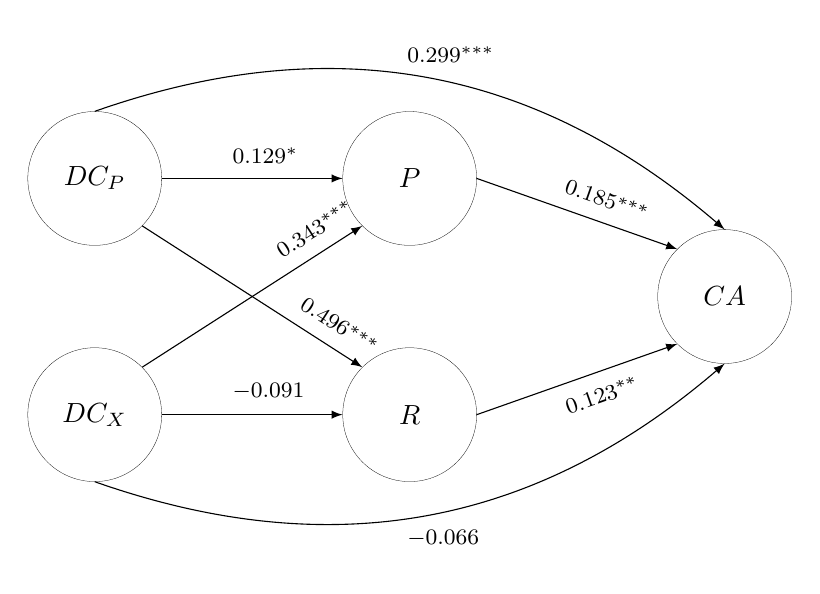
\begin{tikzpicture}
   \centering
   \tikzstyle{mynode}=[circle,draw, ultra thin, draw=black, fill=white, minimum size=17mm,inner sep=0pt, align=center]
        
   \node[mynode] (dc1){$DC_P$};
   \node[mynode,below of=dc1, yshift=-2cm] (dc2){$DC_X$};
   \node[mynode,right of=dc1, xshift=3cm] (or){$P$};
   \node[mynode,right of=dc2, xshift=3cm] (ma){$R$};
   \node[mynode,right of=ma, xshift=3cm, yshift=1.5cm] (ca){$CA$};
   
   
   \draw[-latex] (dc1.east) -- node[text width=0.5cm,font=\footnotesize, above=2pt,align=left,
   fill=white] {$0.129^{*}$} (or.west);

   \draw[-latex] (dc2.east) -- node[text width=0.5cm,font=\footnotesize, above=2pt, align=left,
   fill=white] {$-0.091^{}$} (ma.west);

   \draw[-latex] (dc1.south east) -- node[text width=0.5cm,font=\footnotesize,  above=2pt,
   align=left, fill=white,sloped, near end] {$0.496^{***}$} (ma.north west);

   \draw[-latex] (dc2.north east) -- node[text width=0.5cm,font=\footnotesize, above=2pt,align=left,
   fill=white,sloped, near end]{$0.343^{***}$} (or.south west);

    \draw[-latex] (or.east) -- node[text width=0.5cm,font=\footnotesize, align=left,above=2pt,
   fill=white,sloped]{$0.185^{***}$} (ca.north west);

   \draw[-latex] (ma.east) -- node[text width=0.5cm,font=\footnotesize, below=2pt,
   fill=white,sloped]{$0.123^{**}$} (ca.south west);

   \draw[-latex] (dc1.north)[bend left] to node[text width=0.5cm,font=\footnotesize, above=2pt,align=center,
   fill=white]{$0.299^{***}$}(ca.north);

   \draw[-latex] (dc2.south)[bend right] to node[text width=0.5cm,font=\footnotesize,below=2pt, align=left,
   fill=white]{$-0.066^{}$} (ca.south);
    
 
\end{tikzpicture}
